\begin{figure}[H]
  \begin{center}
    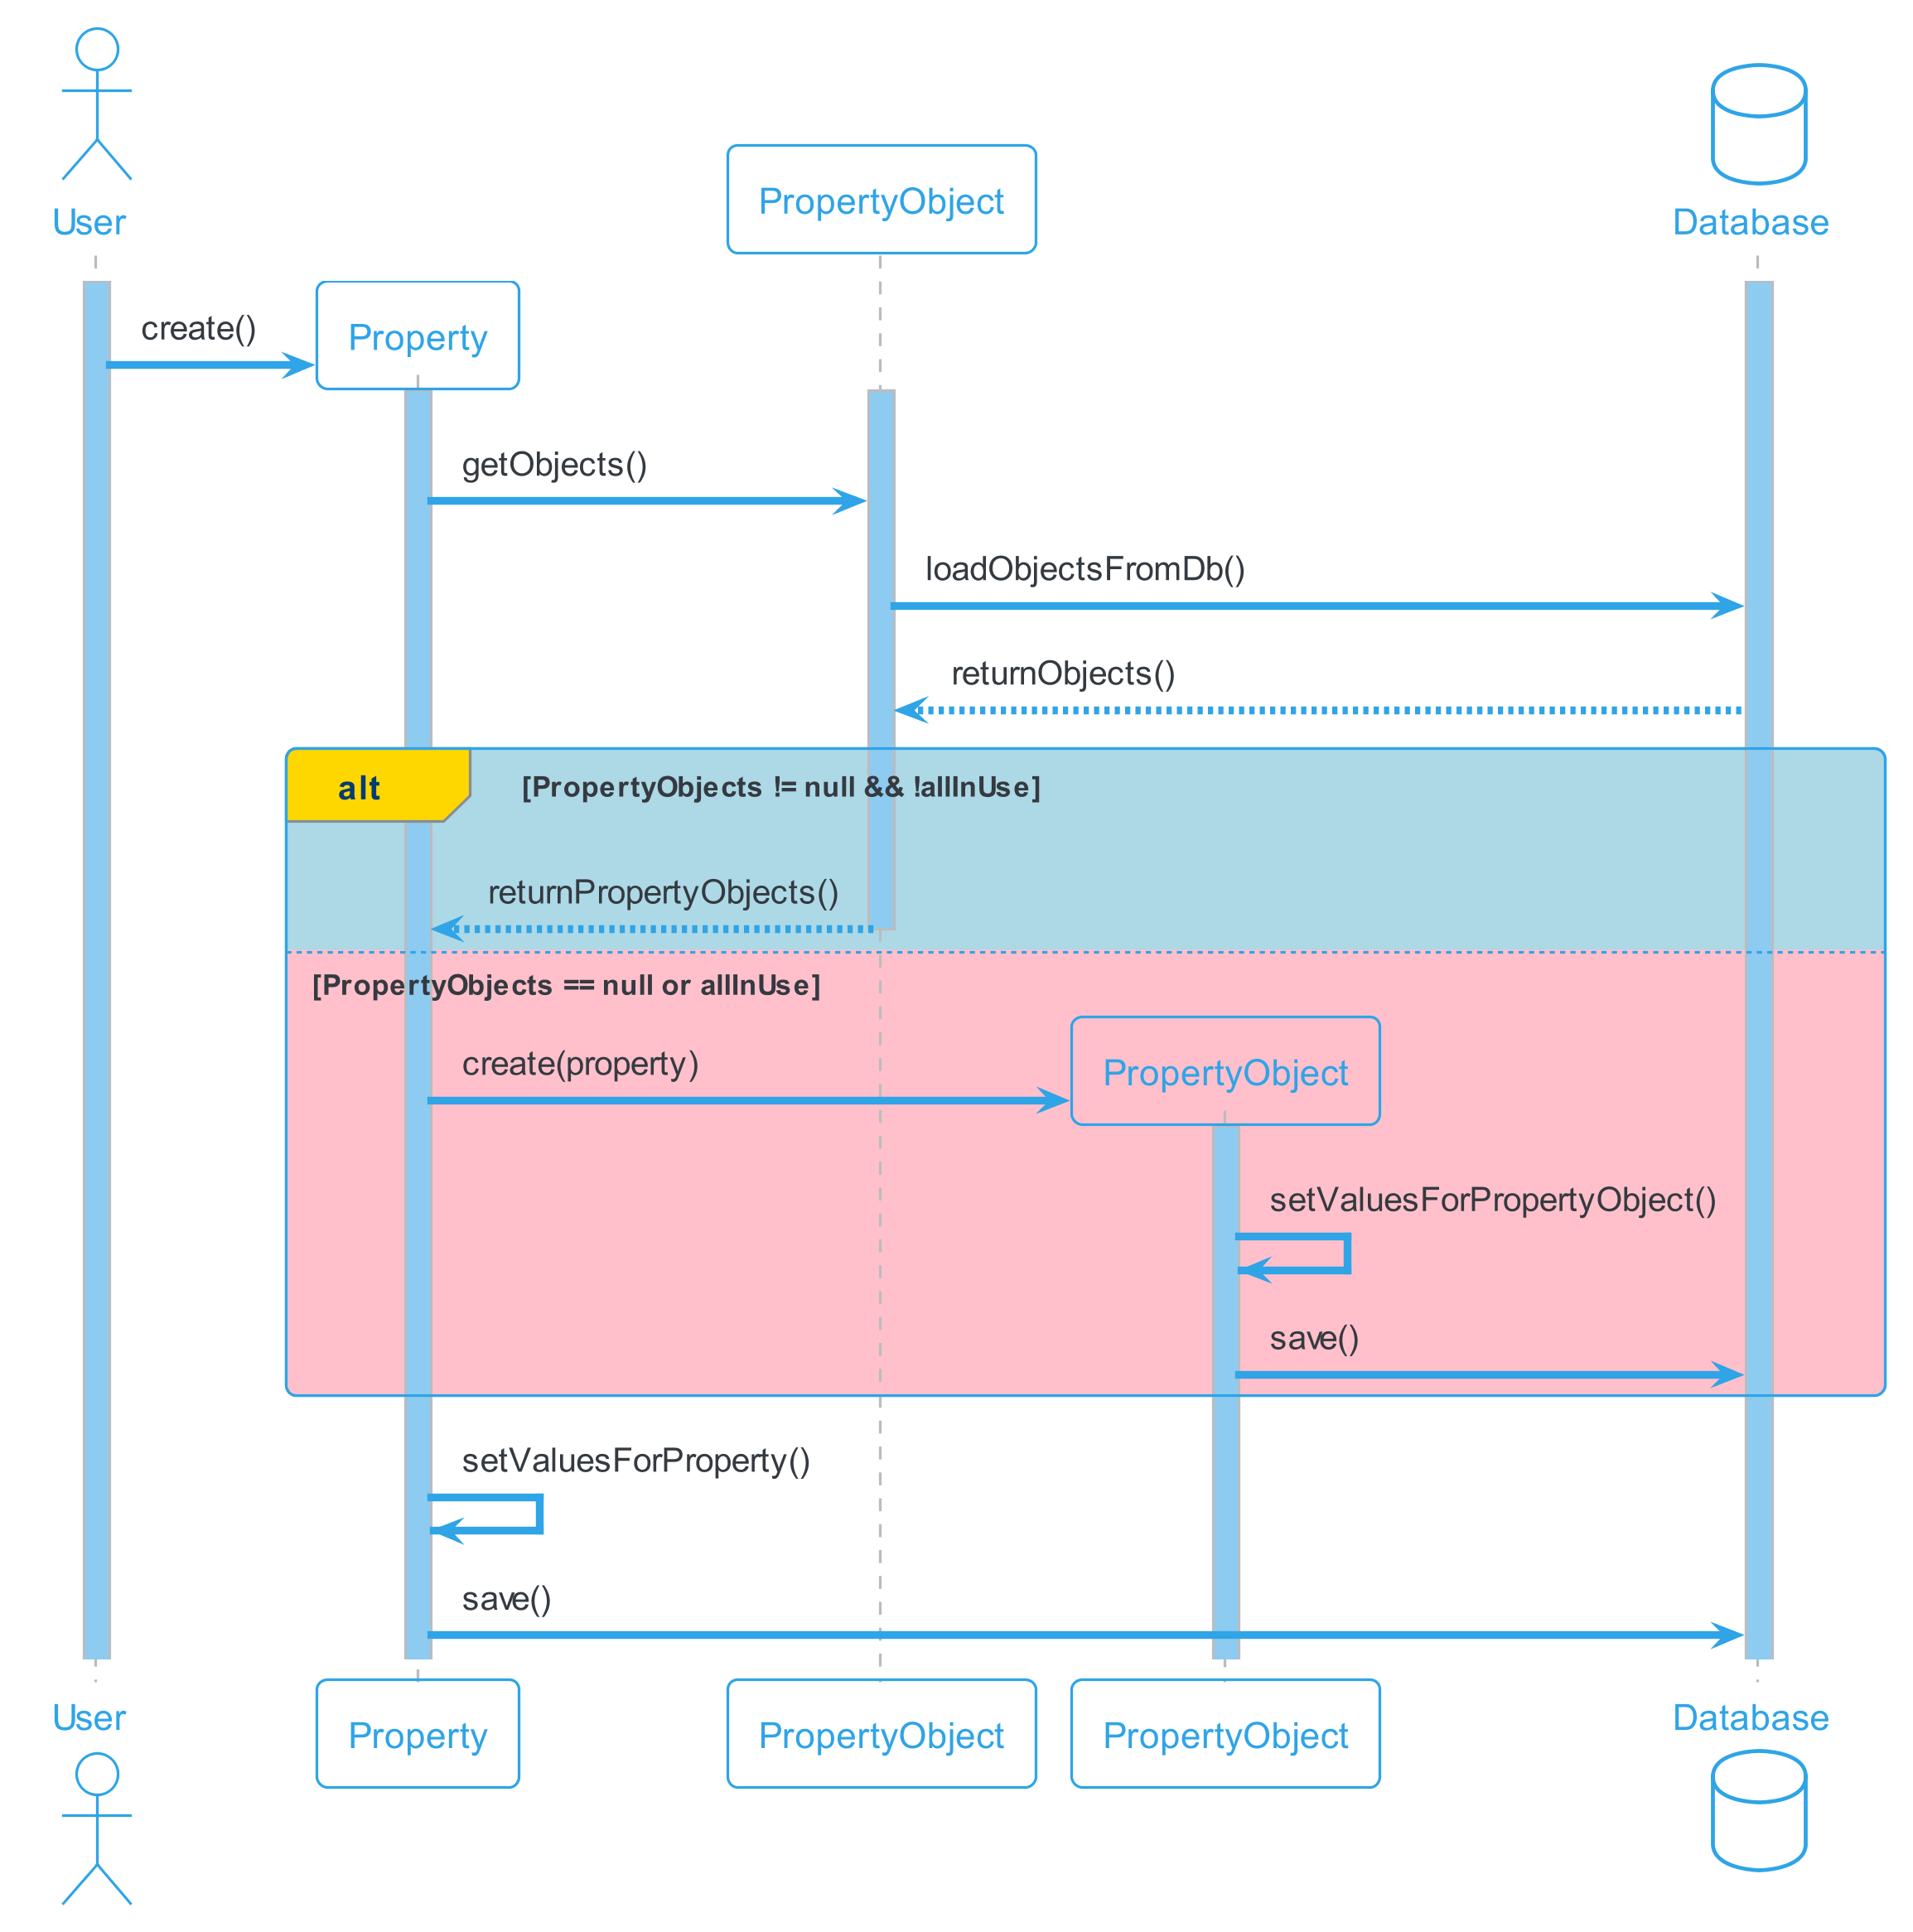
\includegraphics[width=0.5\linewidth]{content/diagrams/out/sequenzdiagram/liegenschaftErfassen/LiegenschaftErfassen.png}
    \caption{SQ-Liegenschaft erfassen}
    \label{sqiegenschaft}
  \end{center}
\end{figure}

\begin{figure}[H]
  \begin{center}
    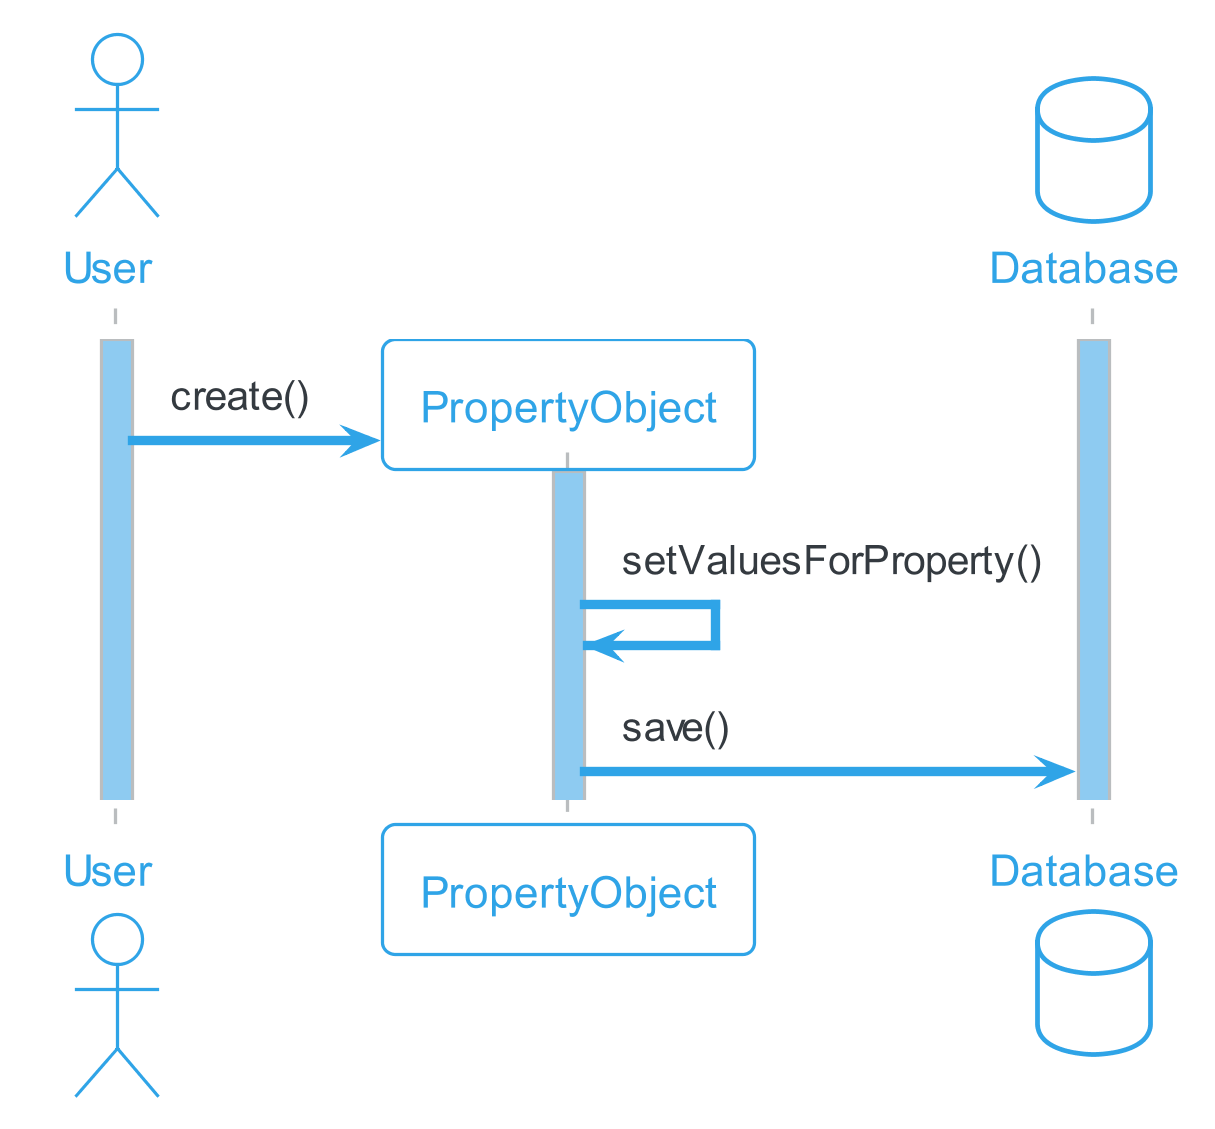
\includegraphics[width=0.5\linewidth]{content/diagrams/out/sequenzdiagram/objektErfassen/ObjekttErfassen.png}
    \caption{SQ-Objekt erfassen}
    \label{sqObjektErfassen}
  \end{center}
\end{figure}

\begin{figure}[H]
  \begin{center}
    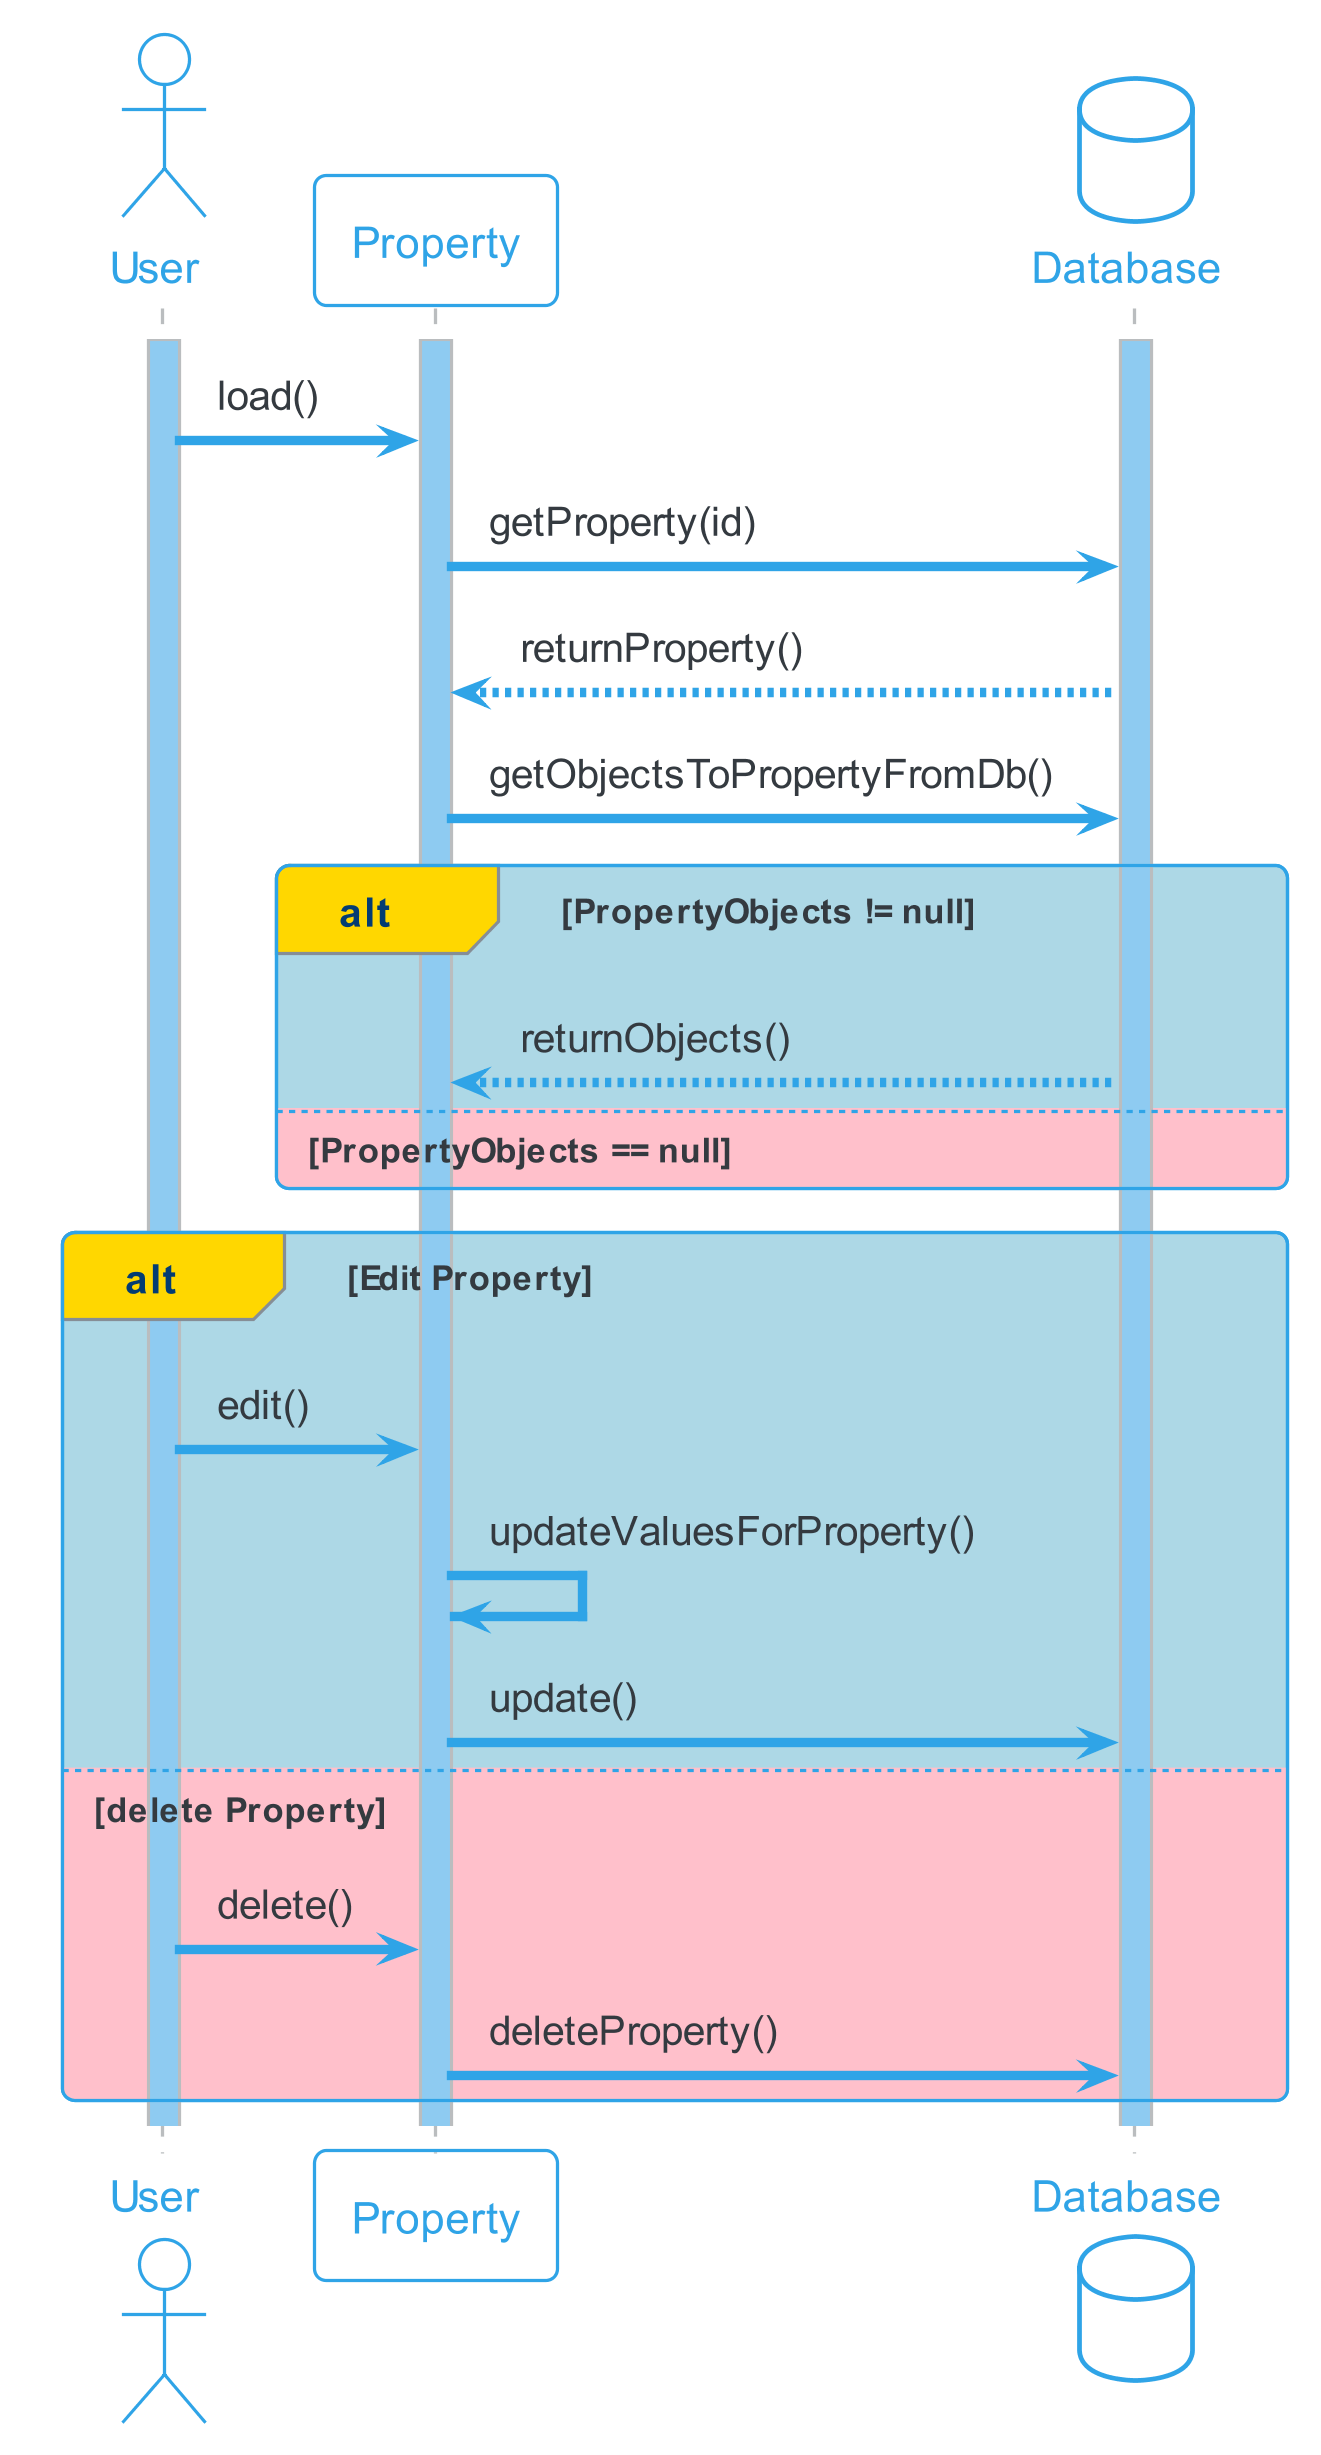
\includegraphics[width=0.55\linewidth]{content/diagrams/out/sequenzdiagram/liegenschaftAnsehenBearbeiten/LiegenschaftAnsehenBearbeiten.png}
    \caption{SQ-Liegenschaft Ansehen/Bearbeiten/Löschen}
    \label{sqOLiegenschatEdit}
  \end{center}
\end{figure}

\begin{figure}[H]
  \begin{center}
    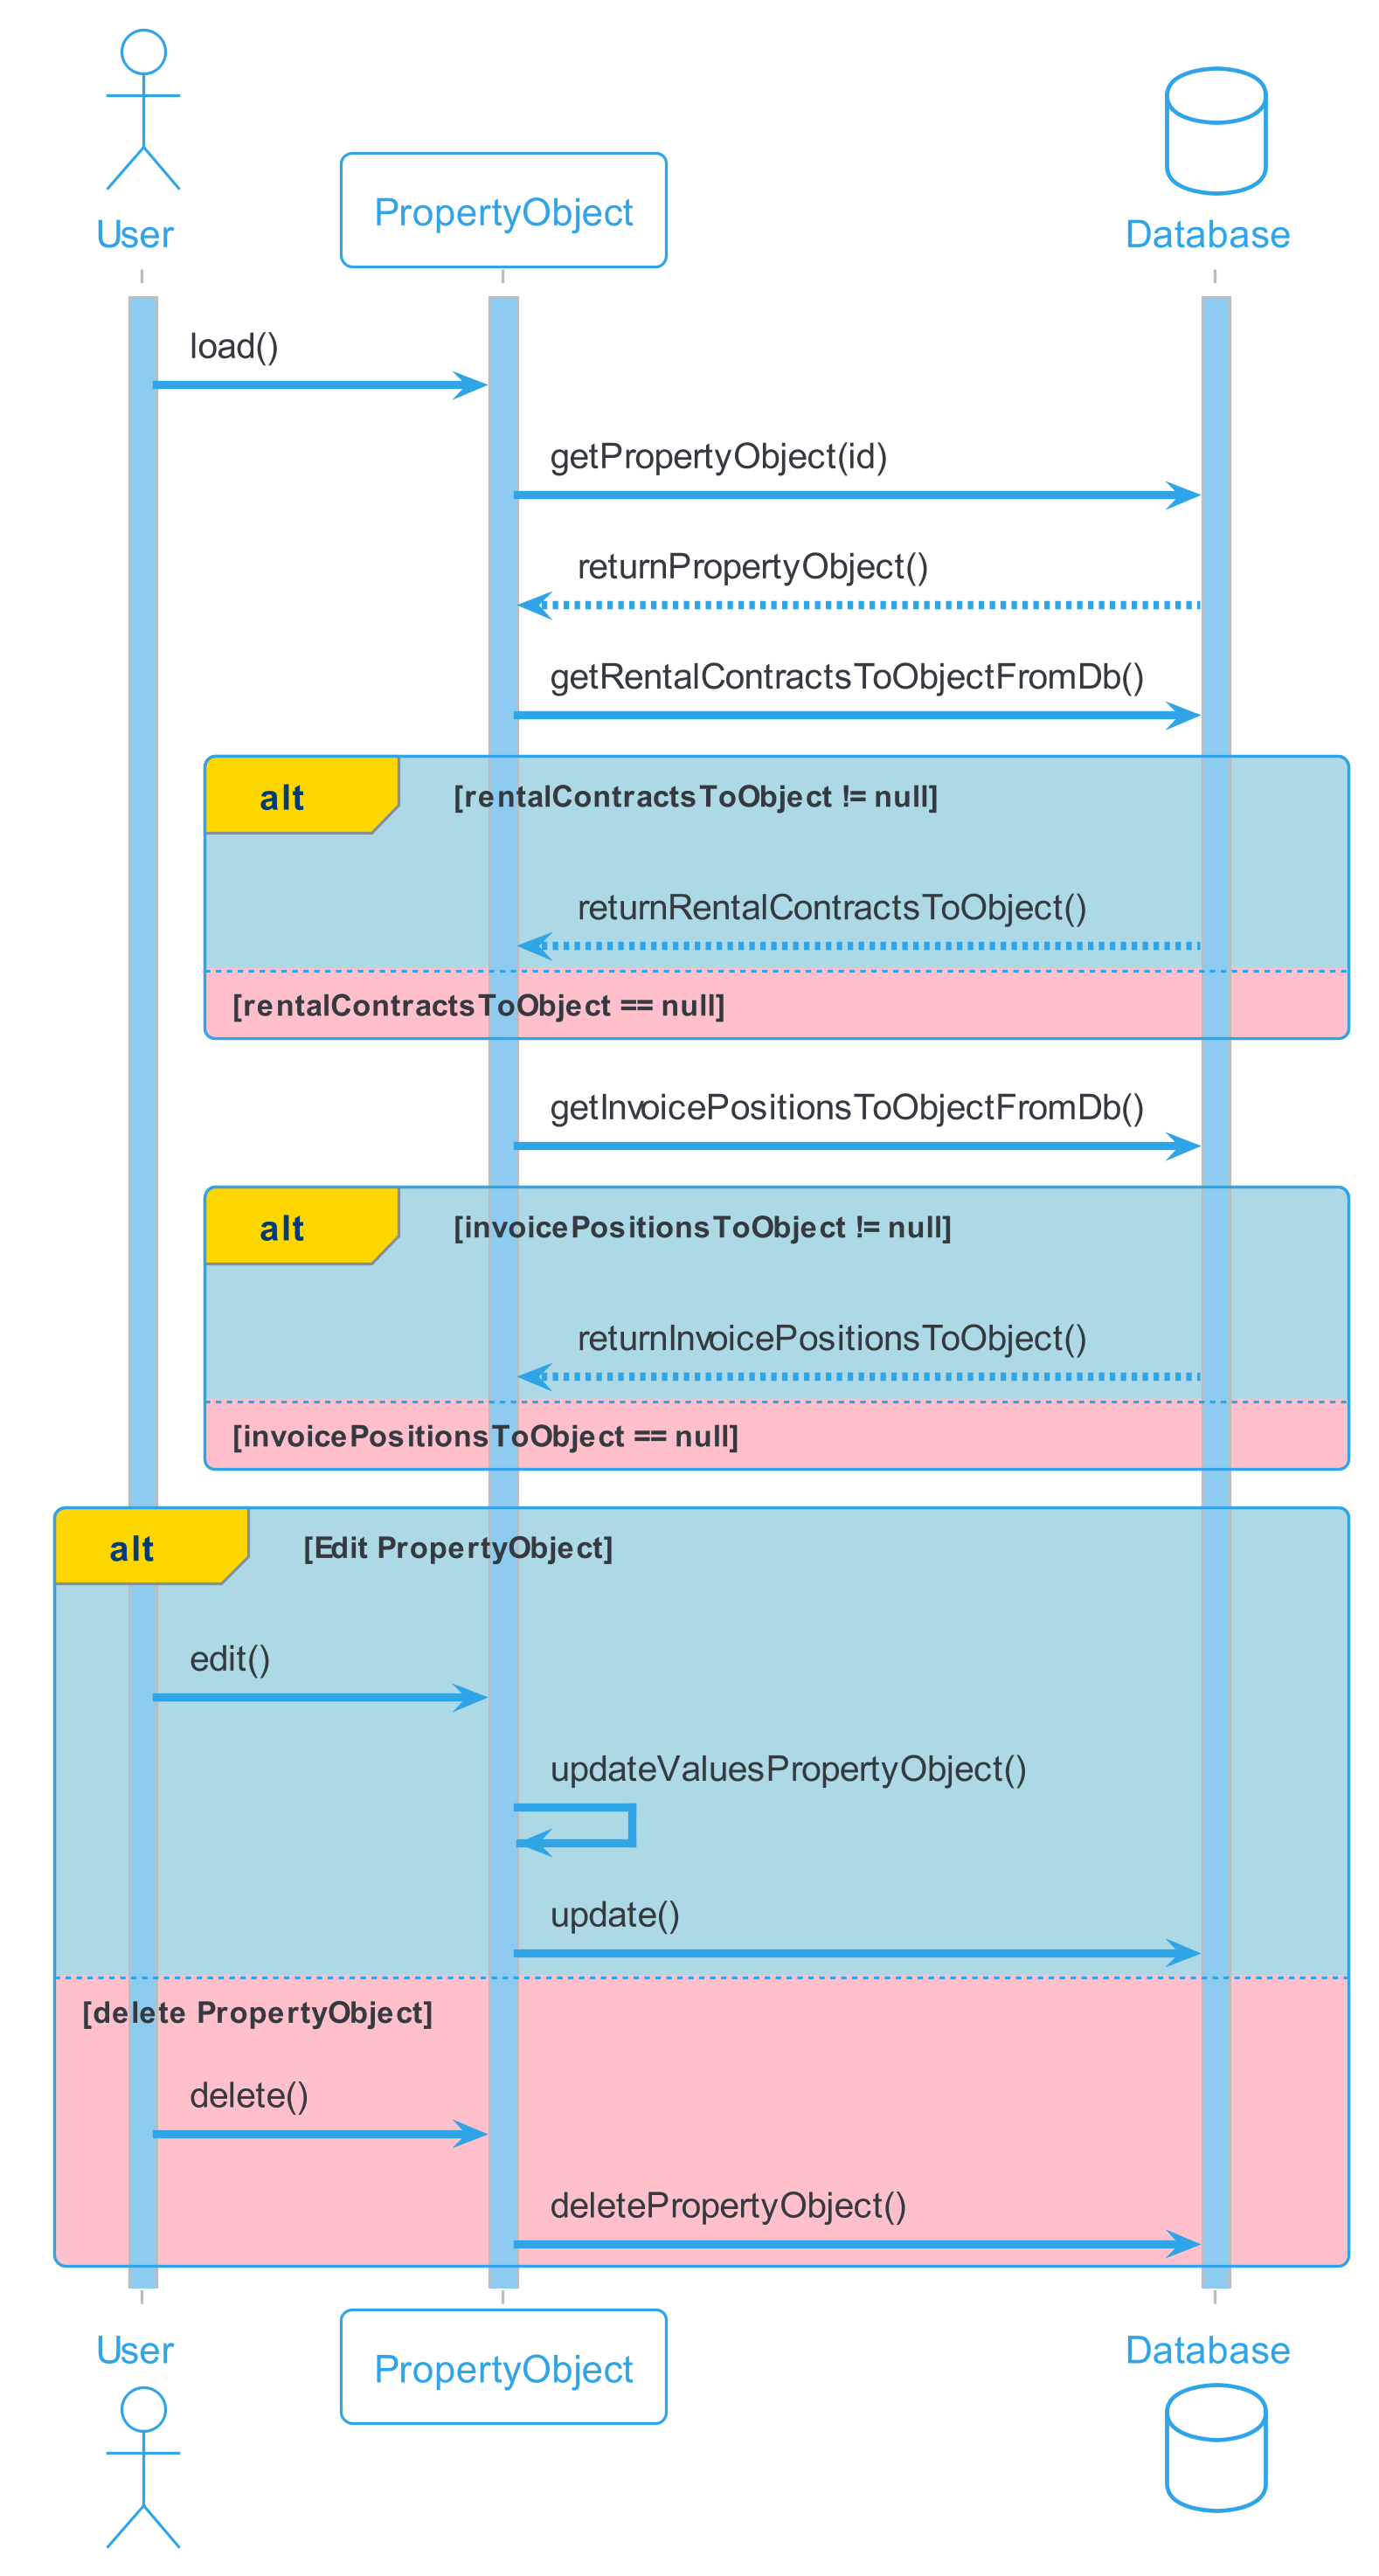
\includegraphics[width=0.7\linewidth]{content/diagrams/out/sequenzdiagram/objektAnsehenBearbeiten/objektAnsehenBearbeiten.png}
    \caption{SQ-Objekt Ansehen/Bearbeiten/Löschen}
    \label{sqObjektEdit}
  \end{center}
\end{figure}

\begin{figure}[H]
  \begin{center}
    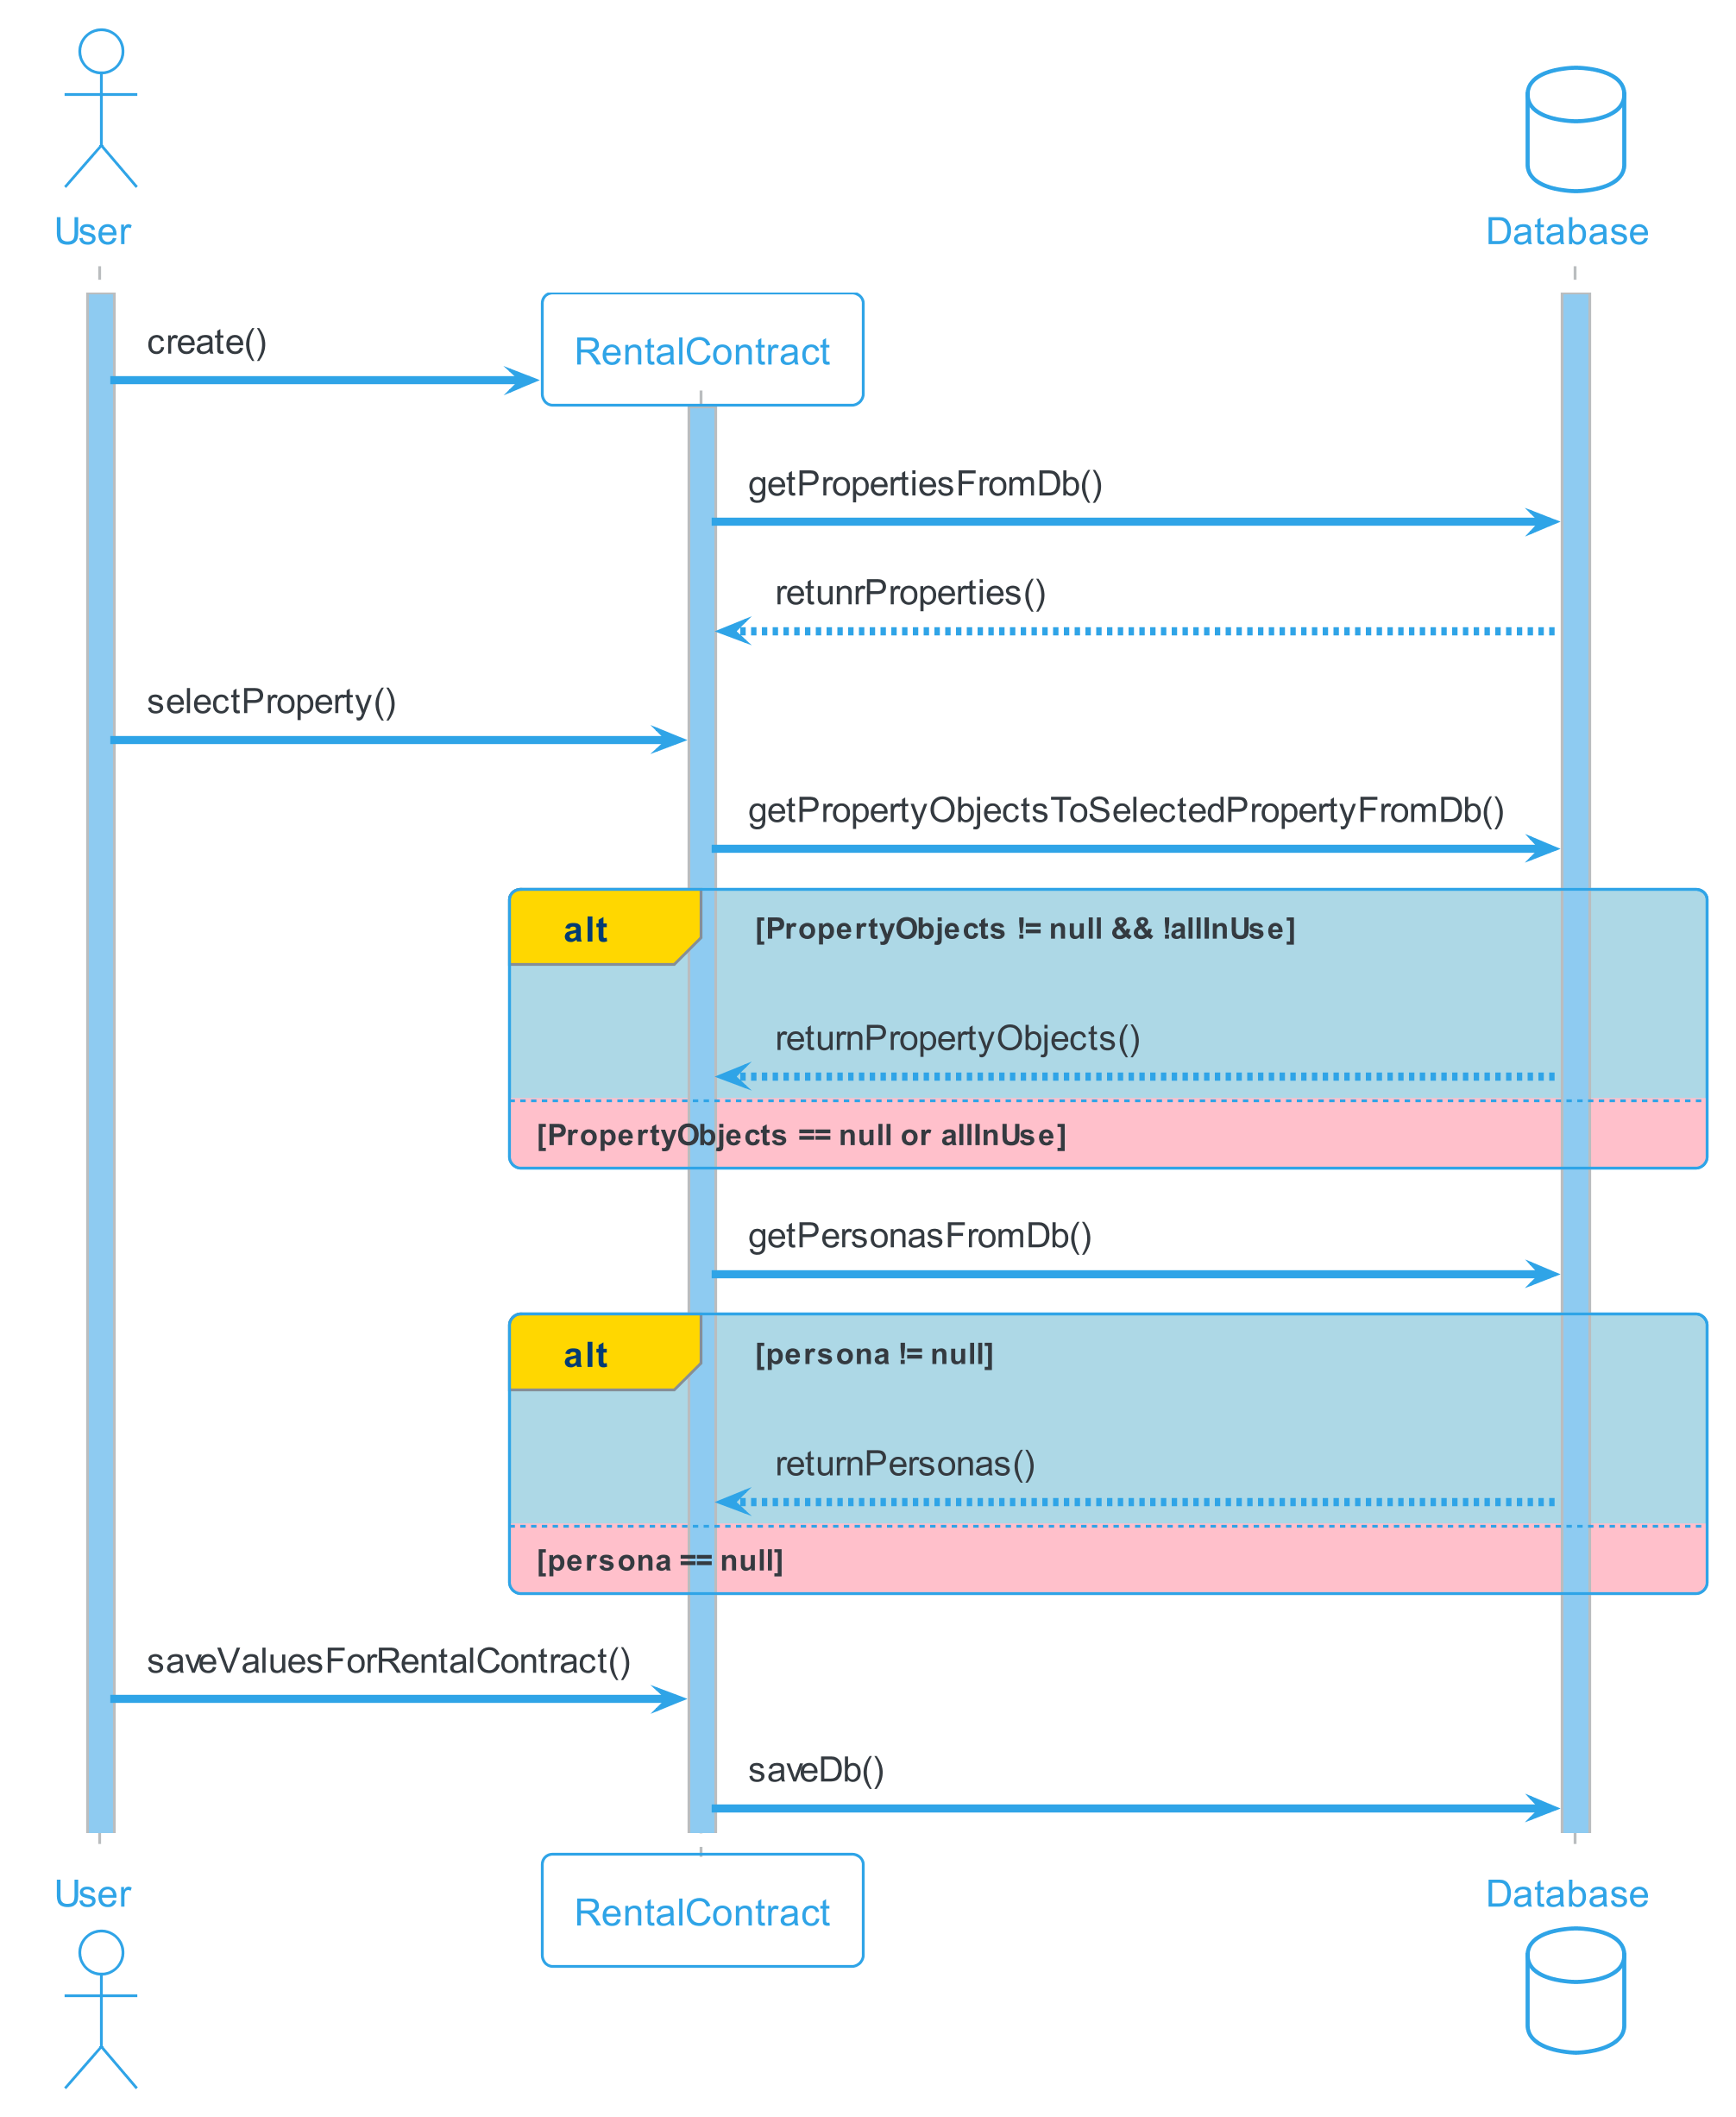
\includegraphics[width=1\linewidth]{content/diagrams/out/sequenzdiagram/mietvertrag/mietvertrag.png}
    \caption{SQ-Mietvertrag}
    \label{sqMietvertrag}
  \end{center}
\end{figure}

\begin{figure}[H]
  \begin{center}
    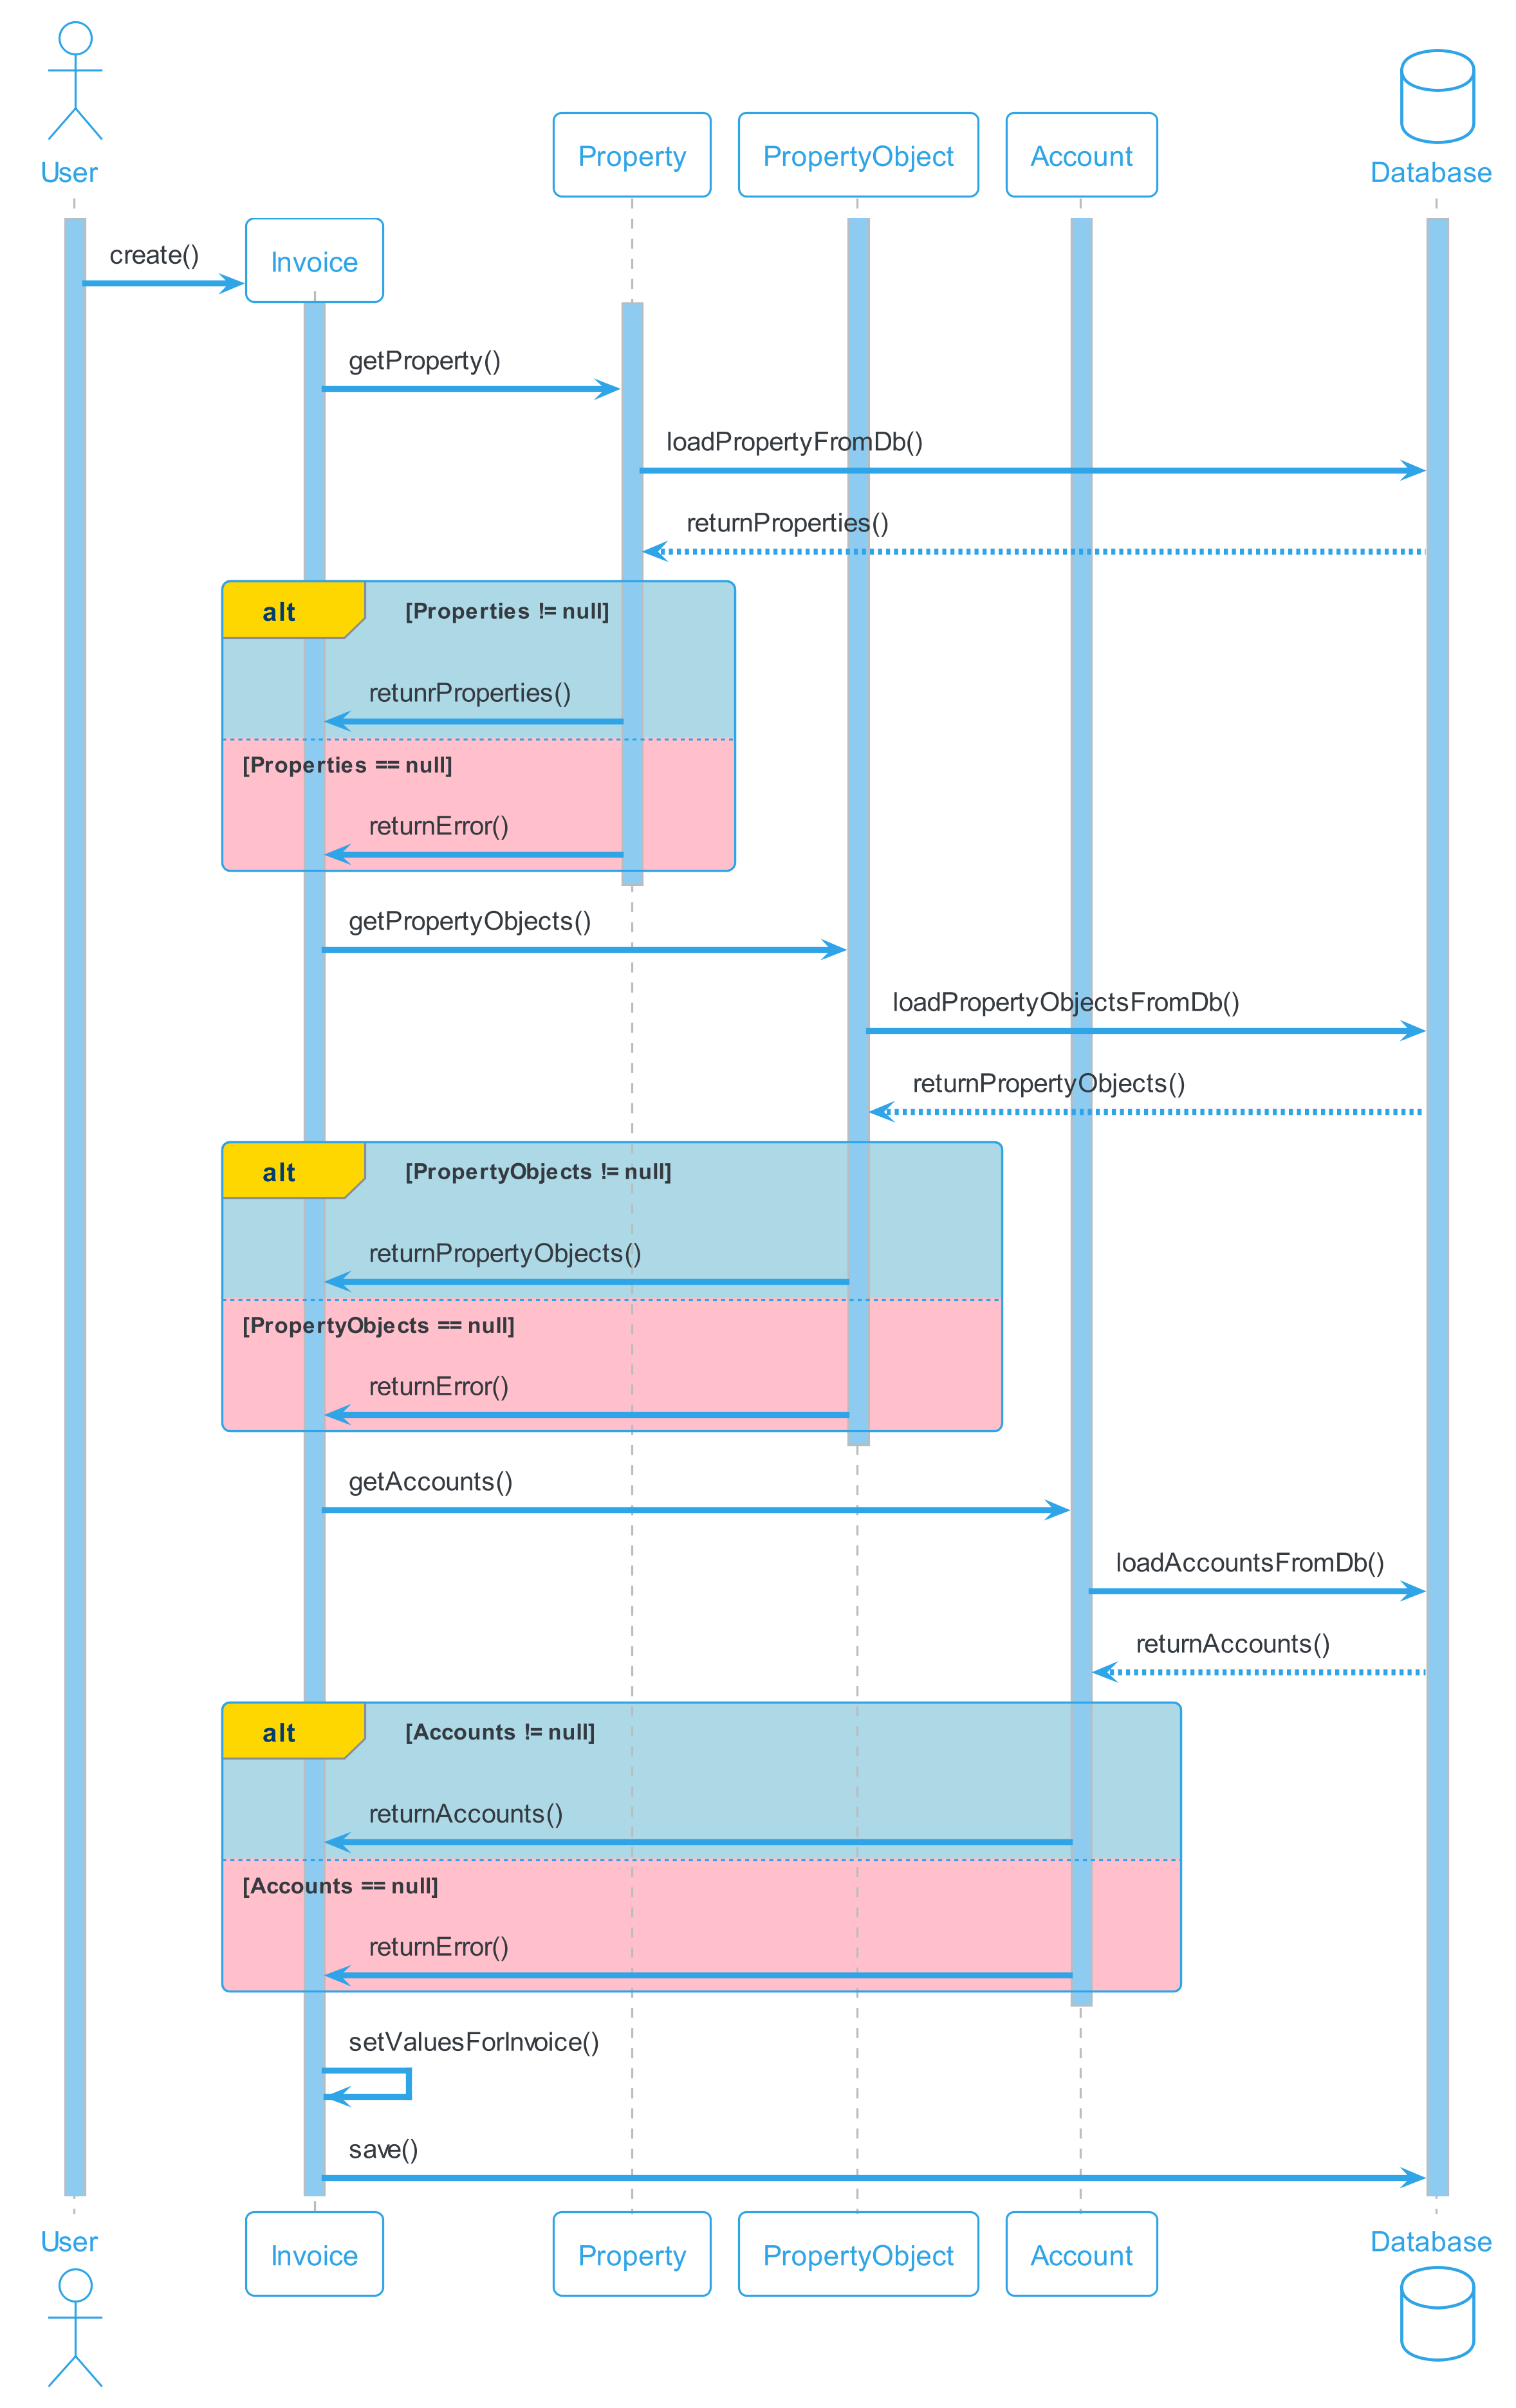
\includegraphics[height=1\textheight]{content/diagrams/out/sequenzdiagram/rechnung/Rechnung.png}
    \caption{SQ-Rechnung}
    \label{sqREchnung}
  \end{center}
\end{figure}